% -*- program: xelatex -*-
\documentclass[compress]{beamer}
\usetheme[usetitleprogressbar]{m}
\setbeamercovered{transparent}
\usepackage{commath}
\usepackage{mathtools}
\usepackage{cleveref}


% bibliography
\RequirePackage{csquotes}
\emergencystretch=1em
\hfuzz=5.002pt 
\RequirePackage[%
backend=biber,                       % use BibTeX
style=chicago-authordate,
url=false, isbn=false, doi=false
]{biblatex}
\addbibresource{../Remote.bib}
\usepackage{silence}
\WarningFilter{biblatex}{Patching footnotes failed}

%% author and title 
\title{No cure no pay --- contracts with limited liability}
\subtitle{}
\date{\today}
\author{Rud Faden}
\institute{University of Copenhagen}

\hypersetup{
pdfauthor = {Rud Faden: rudfaden@gmail.com},
pdfsubject = {No cure no pay --- contracts with limited liability},
pdfkeywords = {contingent contracts, limited liability, health care},
pdfcreator = {LaTeXing}
}

\begin{document}

\maketitle

\section*{Introduction \& Motivation}
\begin{frame}{Introduction}
  \begin{itemize}[<+- | alert@+>]
    \item Health care cost are rising --- there is an interest in increasing productivity
    \item Payment schemes should be constructed to increase output
    \item But most focus seems to be on motivating the ``health organization''
    \item Usually contracts are linear --- per item --- fees or fixed wages
    \item I show that the optimal contract is a non-linear, contingent claim contract
  \end{itemize}
\end{frame}

\begin{frame}[c]{Contingent contracts}
  \begin{itemize}[<+- | alert@+>]
    \item Contingent contracts: payment is conditional on outcome
    \item Well known from real estate and US lawyers
    \item \textcite{Schoonbeek2005No} shows that shows that in the optimal contingent state contract, the physician pays a penalty fees to the principal
    \item In many real life situations, such a contract may no be feasible
    \item Therefore i assume that the optimal contract is subject to limited liability
  \end{itemize}
\end{frame}


\begin{frame}[c]{The plan}
  \begin{itemize}[<+- | alert@+>]
    \item Introduce the model
    \item show that a fixed wage is optimal when effort is observed, and in-optimal if not
    \item Show that the optimal contract is non-linear when effort is unobserved
    \item Future work
  \end{itemize}  
\end{frame}

\section*{The Model}
    
\begin{frame}[c]{Environment I}
  \begin{itemize}[<+- | alert@+>]
    \item The physician is employed by a health organization (hospital/municipal)
    \item The physicians work is measured by observable output $y$
    \item $y$ is random, with density $g(y|e)$ where $e$ is the physicians effort
    \item It is assume that $g(\cdot)$ has a monotone likelihood ratio property
          \[
            \frac{\partial}{\partial y}\left(\frac{g_e(y|e)}{g(y|e)}\right)>0
          \]
          I.e.\ $y$ and $e$ are ``complements''
    \item Effort comes at a cost $C(e)$
  \end{itemize}
\end{frame}

\begin{frame}[c]{Environment II}
  \begin{itemize}[<+- | alert@+>]
    \item The physicians payment is given by $r=R(y,e)$
    \item The physician has a additive and separable utility function $u(r,y)$, which depends on payment and output
    \item Dependence on output allows for a ``caring'' physician
    \item The hospital has a budgetary income $v(y)$ from which it pays the physician
  \end{itemize}
\end{frame}

\begin{frame}[c]{The incentive problem}
  The main problem is to find a contract $r=R(y,e)$, with the property that expected utility of the physician
  \begin{align}
    U(R,e)=\int u(R(y,e),y)g(y|e)\dif y-C(e) \label{eq:phys-util} 
  \end{align}
  cannot be increased by a change in $R(y,e)$, without decreasing the expected net income of the hospital
  \[
    V(R,e)=\int \left[y-R(y,e)\right] g(y|e)\dif y
  \]
  subject to the \emph{incentive constraint} that effort in \cref{eq:phys-util} insures maximal utility
\end{frame}

\begin{frame}[c]{Limited Liability}
  \begin{itemize}[<+- | alert@+>]
    \item A key feature of the model is limited liability
    \item Implies that the physician cannot be forced to pay for bad outcome and the hospital cannot be forced to pay more than the value of output
    \item Formally $0\leq R(y,e) \leq y$
    \item Limited liability reduces the set of contracts
    \item E.g.\ it rules out a \citeauthor{Mirrlees1974Notes} forcing contract
  \end{itemize}
\end{frame}

\begin{frame}[c]{The Formal Problem}
  \begin{subequations}
    \label{eq:khun-tucker-general}
    \begin{align}
      \max_{R,e}   & \int_0^{\infty}\left[u(R(y,e))+\delta y\right]g(y|e)\dif y-C(e)\label{subeq:khun-tucker1-general} \\
      \text{s.t. } & \int_{0}^{\infty} v(y-R(y,e))g(y|e)\dif y\geq y_L^0 \label{subeq:khun-tucker2-general}            \\
                   & E[u(R(y,e),y)|e]\leq E[u(R,e^*)|e] \label{subeq:khun-tucker3-general}                             \\
                   & 0\leq R(y,e)\leq y \label{subeq:khun-tucker4-general}                                             
    \end{align}
  \end{subequations}
  where \cref{subeq:khun-tucker1-general,subeq:khun-tucker2-general} are the physicians and hospitals utility. \cref{subeq:khun-tucker3-general} is the physicians \emph{incentive constraint} and \cref{subeq:khun-tucker4-general} is the limited liability constraint
\end{frame}

\begin{frame}[c]{First-Best and the In-optimality of Fixed Wage I}
  \begin{itemize}[<+- | alert@+>]
    \item When effort is observable the problem becomes
          \begin{align*}
            \max_{R,e}   & \int_0^{\infty}\left[u(R(y,e))+\delta y\right]g(y|e)\dif y-C(e) \\
            \text{s.t. } & \int_{0}^{\infty} v(y-R(y,e))g(y|e)\dif y\geq y_L^0             
          \end{align*}
    \item Using point-wise optimization the optimal contract is implicitly given by 
          \[
            \frac{v'(y-R(y,e))}{u'(R(y,e))}=\frac{1}{\lambda}
          \]
          I.e.\ a fixed wage
    \item This is the \emph{first-best} solution denoted $R_\lambda(y,e)$
  \end{itemize}
\end{frame}

\begin{frame}[c]{First-Best and the In-optimality of Fixed Wage II}
  \begin{itemize}[<+- | alert@+>]
    \item When effort is not observed, and $0\leq R(y,e)\leq y$, the solution is
          \[
            \frac{v'(y-R(y,e))}{u'(R(y,e))}=\frac{1}{\lambda}+\frac{\mu}{\lambda}\frac{g_e(y|e)}{g(y|e)}>R_\lambda(y)
          \]
    \item The optimal contract is now increasing in $y$ by the monotone likelihood ratio
    \item Due to limited liability, even if the physician is risk neutral, the first-best is not achievable
  \end{itemize}
\end{frame}

\begin{frame}[c]{Optimal contract I}
  \begin{alertblock}{Proposition}
    \label{prop:payment-function}
    If $R(y,e)$ solves the maximization problem, then there is some threshold value $y^*$, such that 
    \[
      R^*(y)=\begin{cases}
      0 & \text{for } y< y^* \\
      y & \text{for } y\geq y^*
      \end{cases}            
    \]
    Further,  \textbf{(i)} the hospital is payed according to their participation constraint. \textbf{(ii)}  if the \emph{incentive constraint} binds, then the solution is not the \emph{first-best}. \textbf{(iii)}  if the \emph{incentive constraint} does not bind the first best is achieved.
  \end{alertblock}
\end{frame}

\begin{frame}[c]{The Optimal Contract II}
  \begin{itemize}[<+- | alert@+>]
    \item The rest of the presentation will be a proof of the proposition
    \item I assume that both parties are risk neutral and the utility is additive and separable
    \item $u(\cdot)=R(y,e)+\delta y$ and $v(\cdot)=y-R(y,e)$
    \item 
  \end{itemize}
\end{frame}

\begin{frame}[c]{The Optimal contract III}
  \begin{itemize}
    \item The problem is then\footnote{Note \cref{subeq:khun-tucker3} is now replaced by it's \emph{relaxed} first order condition \parencite[see][for more details]{Rogerson1985FirstOrder}} 
          \begin{subequations}
            \label{eq:khun-tucker}
            \begin{align}
              \max_{R,e}   & \int_0^{\infty}\left[R(y,e)+\delta y\right]g(y|e)\dif y-C(e)\label{subeq:khun-tucker1} \\
              \text{s.t. } & \int_{0}^{\infty} (y-R(y,e))g(y|e)\dif y\geq y_L^0 \label{subeq:khun-tucker2}          \\
                           & \frac{\partial}{\partial e}E[u(R(y,e),y)|e]\geq 0 \label{subeq:khun-tucker3}           \\
                           & 0\leq R(y,e)\leq y \label{subeq:khun-tucker4}                                          
            \end{align}
          \end{subequations}
  \end{itemize}
\end{frame}

\begin{frame}[c]{Optimal Contract IV}
  I can write this in Lagrangian form
  \begin{align}
    \begin{split}
    \mathcal{L}  = & [R(y,e)+\delta y]g(y|e)-C(e)+                   \\ 
                   & \mu [(R(y,e)+\delta y)g_e(y|e)-C_e(e)]+         \\ 
                   & \lambda [(y-R(y,e))g(y|e)-y_L^0]+               \\
                   & \theta(y) R(y,e)+\theta(y)\left(y-R(y,e)\right) 
    \end{split}
  \end{align}
\end{frame}

\begin{frame}[c]{Optimal Contract V}
  The first order conditions are
  \begin{subequations}
    \label{eq:foc}
    \begin{align}
      \frac{\partial}{\partial R} \mathcal{L}=g(y|e)\left[1-\lambda+\mu \frac{g_e(y|e)}{g(y|e)}\right] +\theta(y)-\eta(y) & =0 \label{subeq:foc1} \\
      \frac{\partial}{\partial e} \mathcal{L}=[R(y,e)+\delta y]g_e(y|e)-C_e(e)+ \qquad \qquad \nonumber \\ 
      \mu\left[(R(y,e)+\delta y)g_{ee}(y|e)- C_{ee(e)}\right] \qquad                                                      & \nonumber             \\ 
      +\lambda\left[(y-R(y,e)) g_e(y|e)-y_l^0\right]                                                                      & =0 \label{subeq:foc2} 
    \end{align}
  \end{subequations}
\end{frame}

\begin{frame}[c]{Optimal Contract VI}
  \begin{itemize}[<+- | alert@+>]
    \item Because of non-negativity and complementary slackness conditions for $\theta(y)$ and $\eta(y)$, \cref{subeq:foc1} yields
          \begin{subequations}
            \label{eq:KT-analysis}
            \begin{alignat*}{3}
              \phi(y,e) = g(y|e)\left[1-\lambda+\mu \frac{g_e(y|e)}{g(y|e)}\right]
                        & \: > \: & 0 & \enspace \Rightarrow &   & \enspace R(y,e)=y        \\
              \phi(y,e) & \: = \: & 0 & \enspace \Rightarrow &   & \enspace R(y,e)\in [0,y] \\
              \phi(y,e) & \: < \: & 0 & \enspace \Rightarrow &   & \enspace R(y,e) =0       
            \end{alignat*}
          \end{subequations}
    \item Because $\frac{g_e(y|e)}{g(y|e)}$ is increasing in $y$, $\phi(y,e)$ crosses zero once and from below. I.e.\ $R(y,e)$ is $0$ for some $y<y^*$ and $y$ for $y>y^{*}$
  \end{itemize}
\end{frame}

\begin{frame}[c]{Optimal Contract VII}
  \begin{columns}
    \column{0.5\linewidth}
    \centering
    \begin{figure}[htbp]
      \centering
      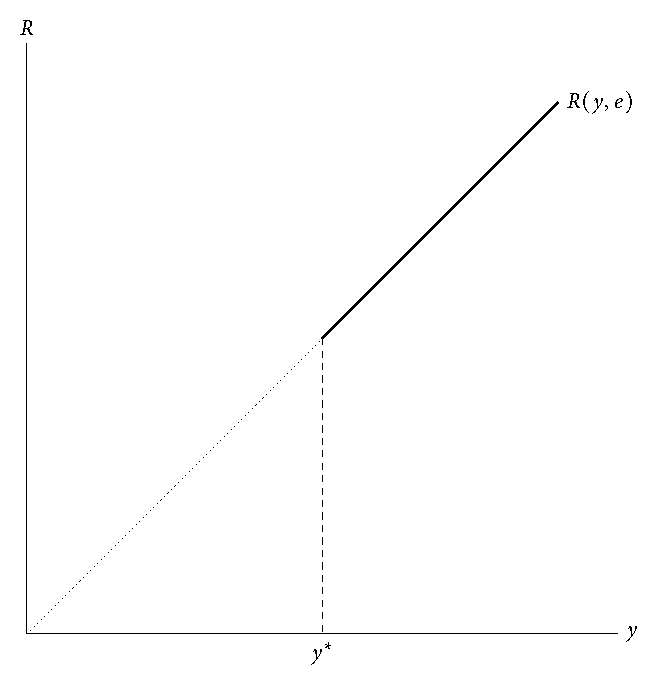
\includegraphics[width=1\textwidth]{../../fig/optimal-R.pdf}
    \end{figure}
    \column{0.5\linewidth}
        
    \textbf{intuition:} By moving payment from low outcome states to high outcome states, forces the physician to commit to higher effort levels
  \end{columns}
\end{frame}

\begin{frame}[c]{Optimal Contract VIII}
  \begin{itemize}
    \item To proof (i) that $y=y_L^0$ note that 
          \begin{align}
            \frac{\partial}{\partial e} \mathcal{L}=\overbrace{[R(y,e)+\delta y]g_e(y|e)-C_e(e)}^{=0}+ \qquad \qquad \nonumber \\ 
            \mu\overbrace{\left[(R(y,e)+\delta y)g_{ee}(y|e)- C_{ee(e)}\right]}^{<0} \qquad & \nonumber \\ 
            +\lambda\left[(y-R(y,e)) g_e(y|e)-y_l^0\right]                                  & =0        
          \end{align}
    \item So $\lambda\left[(y-R(y,e)) g_e(y|e)-y_l^0\right]>0$ which implies that $\lambda>0$ and the constraint binds
  \end{itemize}
\end{frame}

\begin{frame}[c]{Optimal Contract IX}
  \begin{itemize}[<+- | alert@+>]
    \item to proof (ii), that the optimum is below the \emph{first-best}, note from (i) it follows trivially that $y\in [0,y]$
    \item Thereby I can write the contract as 
          \[
            R(y,e)=\frac{1}{\lambda}+\frac{\mu}{\lambda}\frac{g_e(y_L^0|e)}{g(y_L^0|e)}>R_\lambda(y)
          \]
    \item From this, it is easy to see that if the \emph{incentive constraint} does not hold ($\mu=0$), then the first best is achieved.
  \end{itemize}
\end{frame}

\begin{frame}[c]
  \frametitle{Future work}
  \begin{itemize}[<+- | alert@+>]
    \item Analyze the problem when the agent is risk averse
    \item Look at change in effort when the physicians ``caring'' changes
    \item 
  \end{itemize}
\end{frame}
% bibliography
\begin{frame}[c]{Bibliography}
  \printbibliography%
      
\end{frame}
\end{document}
